\documentclass{article}
\usepackage[utf8]{inputenc}

%%%%% correct style for numeric cites and bibliography
\usepackage[square,numbers]{natbib}
%\bibliographystyle{abbrvnat}
\bibliographystyle{unsrt}
%%%%%%%%%%%%%%%%%%%%%%%%%%%%%%%%%%%%%%%%%%%

% lower margin to 2cm if page count is too long
%\usepackage[margin=2.5cm]{geometry}
\usepackage[letterpaper,top=2cm,bottom=2cm,left=2cm,right=2cm,marginparwidth=1.75cm]{geometry}

\usepackage{multicol}
\setlength\multicolsep{5pt}

\usepackage{parskip}
\setlength{\parindent}{2em}
\usepackage{graphicx}
\usepackage{float}
\usepackage{tabu}
\usepackage{booktabs}
\usepackage{makecell}
\usepackage{multirow}
\usepackage{wrapfig}
\usepackage{indentfirst}
\usepackage{threeparttable}

\usepackage[dvipsnames]{xcolor}
\usepackage{hyperref}
% \newcommand{\todo}[1]{}
% \newcommand{\todoOther}[1]{}
% \newcommand{\Xavier}[1]{}
\newcommand{\todo}[1]{\textcolor{red}{#1 }}
\newcommand{\todoOther}[1]{\textcolor{blue}{#1}}
\newcommand{\Xavier}[1]{\textcolor{OliveGreen}{Xavier: #1}}
\usepackage{soul}
\setstcolor{red}

\usepackage{longtable}

\title{COMP 551 Final Project\\``Size isn't everything, it's what you (can) do with it that counts":\\
a comparison of SqueezeNet and AlexNet}

\date{April 17, 2019}
\author{
  Xavier Morin Duchesne\\
  \texttt{260760216}
  \and
  Bahare Samadi\\
  \texttt{260556423}
 \and
  Gordon Krieger\\
  \texttt{119005244}
}
\begin{document}


\maketitle

\begin{abstract}
We examine the deep learning neural network model SqueezeNet. Improvement in deep learning networks sometimes comes at the expense of size; increasing the depth or width of a network can often give an increase in performance. SqueezeNet is an attempt to move in the other direction: produce a small network that optimizes for size, while keeping an acceptable baseline accuracy. We confirm the main claim of the paper of having AlexNet-level accuracy. We also perform multiple ablation studies of SqueezeNet's architecture: our main finding is that adding a batch normalization layer to SqueezeNet's Fire modules gives a measurable increase in performance. 

\end{abstract}

%\todo{me todo:  discussion cites?}

%\todo{\textbf{Should we consider putting this in a limitations section after the discussion?}}



%\todoOther{General Notes:\\- can we get at least one graph? Of something? Tables are important but not hugely sexy \Xavier{Agreed. Working on having at least one for Aim #2: SqueezeNet vs AlexNet.}\\- page limit is 8 pages, not counting references or an appendix, so we are doing okay, there may still be some overly wordy parts\\- It is not necessary to cite the SqueezeNet paper each time it is mentioned\\- Please remember that AlexNet is an accuracy (and size) baseline only, other than them both being CNNs they have little in common\\- Thanks everyone for working so hard, it's a relief after several frustrating assignments for things to start to come together.}

% \todoOther{Wednesday notes (old notes commented out):\\- Can the grid search parameter tables go in the Appendix? Page space is scarce\\- Tables A2 and A3 need ``accuracy (\%)" added"\\- Please try to be concise: there are a few paragraphs that are quite long and chatty}

% \Xavier{\\
% (1) Tables: I would prefer not. For the large tables, it makes sense to me, but not for the smaller ones. If we're really that starved for space, I first would consider wrapping text around the figures, moving them to the appendix, or even removing ones that are less necessary.\\
% (2) Regarding figures, figures 1 and 2 aren't referenced anywhere as far as I can tell. Is that supposed to be the case?\todo{They are both referenced in section 2, although without using ref labels}\Xavier{Please add ref labels then and please consider wrapping text around them or adding them to the appendix.}\\
% (3) When I'm done writing (hopefully soon...), I'm going to go over the text I have written to see what I can cut down on.\\
% (4) If we really don't have a choice, then, yes, obviously, we can put the tables in the Appendix. Again, however, I would prefer considering other solutions such as wrapping text around them first.
% }

\section{Introduction}

The aim of this study is to investigate the neural network model SqueezeNet, as presented in Iandola et al., ``SqueezeNet: AlexNet-level accuracy with 50x fewer parameters and $<$ 0.5 MB model size" \cite{iandola2016squeezenet}.

The main motivation behind SqueezeNet is to create a neural network design with a small model size. The advantages of small models are made clear in the paper itself: among other things, smaller models require less memory to store, and less bandwidth to transmit. A model with total size of less than a megabyte, as the authors claim for their model, would lend itself to storage on a chip for embedded use. (Two of SqueezeNet's authors, Forrest Iandola and Kurt Keutzer, are founders of a company applying deep learning to the auto industry.) SqueezeNet has since been applied to various learning domains, such as pedestrian detection \cite{verbickas2017squeezemap}, video classification \cite{nanfack2018squeeze}, medical imaging \cite{mohanraj2019hybrid, betancourt2018automatic} and internet of things (IoT) \cite{motamedi2016fast}.

We verify the main claim of the paper, that SqueezeNet can meet the same level of accuracy as AlexNet \cite{krizhevsky2012imagenet} for some visual classification tasks. We trained both models from scratch, although time and computational constraints meant using a smaller dataset than the ImageNet Large Scale Visual Recognition Challenge \cite{imagenet} dataset used in the SqueezeNet paper. We opted instead to use the CIFAR-10 dataset \cite{CIFAR-10}; details are given in section 4.1.

We performed multiple ablation studies to gain insight into SqueezeNet both at 
the broader achitectural level in terms of the number of network layers, as well as the micro-architectural details of SqueezeNet's Fire modules, which form the basic building blocks of the network. Most interestingly, we find that adding a batch normalization \cite{ioffe2015batch} layer to the modules helps increase performance with little additional cost. 

%\todo{mention transfer learning, or don't}

\section{SqueezeNet}
\subsection{Background}

A common approach to improving the accuracy of a convolutional neural network (CNN) is increase the size of the network, for example by adding more layers \cite{goodfellow2016deep}. But this approach has costs for the size needed to store the network, and the number of operations required for training and prediction. SqueezeNet is an attempt to go in the other direction: shrink the network, while maintaining a baseline level of accuracy. 
The baseline in this case is AlexNet \cite{krizhevsky2012imagenet}. AlexNet is best known for its breakthrough performance in the 2012 edition of the ImageNet Large Scale Visual Recognition Challenge \cite{imagenet}. It was the the first CNN do to so, and helped foster the current interest in deep learning models. All subsequent ImageNet competitions have been won by some CNN model. AlexNet's accuracy is no longer state of the art: models exist with better accuracy. Some, such as VGG \cite{vgg}, have many more parameters, although a few, such as Google's Inception network, have fewer. 

\subsection{SqueezeNet model design}

%\todo{I cleaned up a few grammatical mistakes here, and converted a few things to point form where I found it hard to follow. We also need to start cutting for length somewhat. But omg, thank you for writing this section, this would have killed me }

In this section, we go through the Iandola et al. \cite{iandola2016squeezenet} study and explain their proposed model. The main objective of SqueezeNet's architecture is to optimize for parameter count, building a small model that meets an acceptable level of accuracy. They mention three main strategies to meet this goal:
\begin{itemize}
\item 1. Replace (some) 3x3 filters with 1x1 filters. This leads to fewer parameters and works as a means of dimensionalty reduction.  In the filter space, 1x1 convolution acts like coordinate-dependent transformation \cite{kim2016pvanet}. %\todo{in what sense is it coordinate dependent if it ignores spatial information?}
\item 2. Decrease the number of inputs to 3x3 filters. This again decreases the total parameter count. 
\item 3. Downsample late in the network (closer to the output layer). This is an attempt to maximize accuracy on a limited parameter budget. In a convolutional network, each layer produces an output feature map, the size of which is determined by the the size of the input data and the choice of layers. Downsampling in a CNN is typically achieved by setting stride greater than 1 in a convolutional filter. Doing this early in a network leads to smaller feature maps; in SqueezeNet downsampling is performed later in the network, with the intuition that larger feature maps can lead to greater classification accuracy, something strongly suggested in a study by He \& Sun \cite{he2015delving}. 
\end{itemize}

SqueezeNet's Fire module implements all three of these strategies. It is a repeatable building block of the network, consisting of a squeeze convolutional layer (of 1x1 filters) to reduce the parameters i.e. implementing strategy 1, an expand layer that has a mix of 1x1 and 3x3 convolutional filters. The microarchitecture and macroarchitecture of SqueezeNet are shown in Figures~\ref{fig:Figure1} and~\ref{fig:Figure2}, respectively. It is composed of 8 Fire modules (numbered 2-9) and 2 convolutional layers, maxpooling layers, and a final global average pool before a softmax activation function. SqueezeNet performs maxpooling with a stride of 2  after layers conv1, fire4, fire8 and conv10 as part of the third strategy above.

% If you want the figure to be *exactly* here, use H
% \begin{figure}[ht]
\begin{wrapfigure}[13]{r}{0.5\textwidth}
    \vspace{-3em}
    \centering
    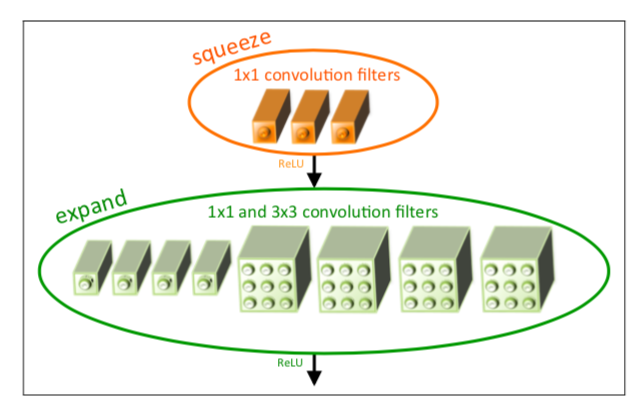
\includegraphics[scale=0.4]{Micro.png}
    \caption{Microarchitectural view: Organization of convolution filters in the Fire module.\cite{iandola2016squeezenet}}
    \label{fig:Figure1}
\end{wrapfigure}
% \end{figure}

Dropout \cite{srivastava2014dropout} with a ratio of 0.5 is applied after the final Fire module. To evaluate the accuracy of SqueezeNet, Iandola et al. used AlexNet as a comparison baseline, settling on a initial learning rate \cite{mishkin2017systematic} of 0.04, with subsequent linear decay. They reported that with a model 50x smaller than AlexNet \cite{krizhevsky2012imagenet}, they achieved the same top-1 and top-5 accuracy on ImageNet. They also report that SqueezeNet can undergo significant size compression without accuracy loss; we address this more in section 4.7. 

%\todoOther{The 510x claim is misleading, since this compares compressed SqueezeNet to \emph{uncompressed} AlexNet. The compressed models are only 14.5x apart}


\begin{figure}[ht]
    \centering
    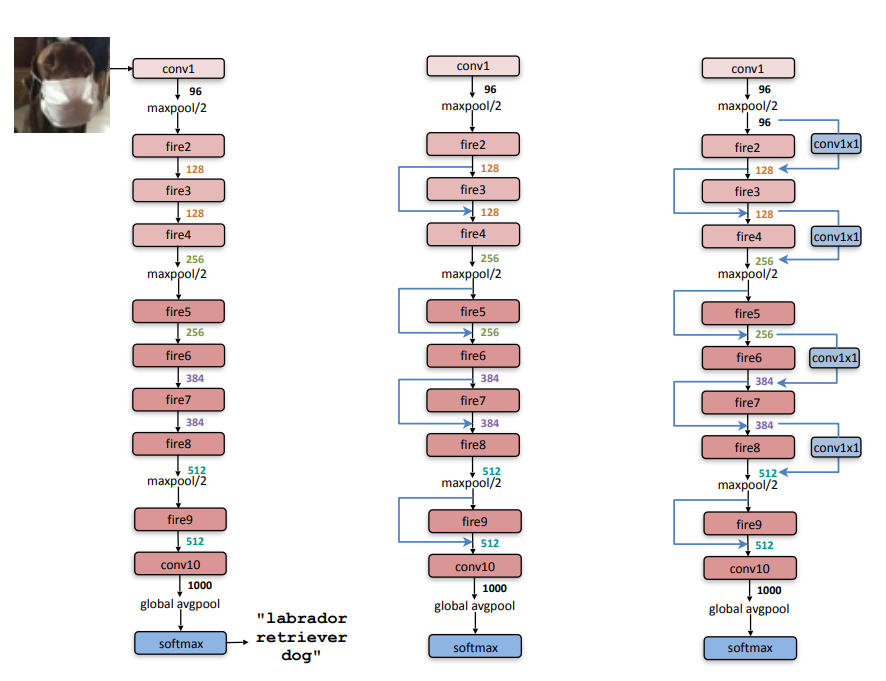
\includegraphics[scale=0.5]{Macro.png}
    \caption{Macroarchitectural view of the SqueezeNet architecture. Left: SqueezeNet; Middle: SqueezeNet with simple bypass; Right: SqueezeNet with complex bypass.\cite{iandola2016squeezenet}}
    \label{fig:Figure2}
\end{figure}

% \todoOther{Do we want Figure 2? It shows part of the paper we're ignoring. I think fig 1 is good though}
% \todoOther{It is in the part explaining the SqueezeNet model, so I think it might be useful and then we say that we did not use this part when we modified the model, but if you think we should not, you can remove it}


%\section*{The impact of CNN architectural choices on model size and accuracy in both microarchitectural and macroarchitectural design}
%better title?
\subsection{Architectural considerations}

%\todo{I cut this into paragraphs, and tried to clarify a few issues I found hard to understand. Is this section too long? Can the main points be mentioned in the previous section instead? Arguably our main concern in our paper is verification and testing, but this section concerns only how the authors came up with the model.}

The ``micro-architectural" details of SqueezeNet concerns the construction of the Fire module. Each module has three hyperparameters: $s_{1x1}$, the number of 1x1 filters in the initial ``squeeze" layer, $e_{1x1}$, the number of 1x1 filters in the second, ``expand" layer, and $e_{3x3}$, the number of 3x3 filters, all in the expand layer. The eight Fire modules have 24 such parameters between them. Figure~\ref{fig:Figure2} shows an example module with a squeeze layer of three 1x1 filters, followed by an expand layer of four 1x1 and 3x3 layers each.

The authors define a \emph{squeeze ratio} (SR) as the ratio between the number of filters in squeeze layers and the number of filters in expand layers. By varying the architecture, the authors found that increasing SR beyond 0.125 can increase the level of the accuracy on ImageNet around from 80.3 \% to 86\%, but increases the model size from 4.8MB to 19MB. Accuracy peaks at 86\% at SR = 0.75. Adding more 3x3 filters leads to a larger model without any improvement in accuracy on ImageNet. Fire modules in SqueezeNet vary in size, but all have SR = 0.125 (note that the image in Fig~\ref{fig:Figure1}, drawn from the SqueezeNet paper, actually shows SR = 0.375).

Macro-architectural experiments in the SqueezeNet paper involve adding bypass connections between layers in the network. The motivation here is to allow a means for information to pass through the network that might otherwise be squeezed out by the Fire modules. The authors explore both ``simple" and ``complex" connections (see Fig.~\ref{fig:Figure2}). Simple connections just repeat the outputs of previous layers later in the network, this requires matching input and output sizes between non-consecutive modules. Complex connections add a convolution to the connection between layers: input and output sizes need not match, but this adds further parameters to the network.  In experiments the authors found that simple bypass lead to greater improvement than complex ones. 
%this is repeated from above
%Considering all of the mentioned parameters for the CNN architecture as SqueezeNet, it was concluded in \cite{iandola2016squeezenet} that this model with 50X fewer parameters can compete with the AlexNet in terms of accuracy on ImageNet.


%\todo{Recommendations from "Systematic evaluation of CNN advances on the ImageNet" \cite{mishkin2017systematic} : A summary of recommendations: 
%• use ELU non-linearity without batchnorm or ReLU with it.
%• apply a learned colorspace transformation of RGB.
%• use the linear learning rate decay policy.
%• use a sum of the average and max pooling layers.
%• use mini-batch size around 128 or 256. If this is too big for your GPU, decrease the learning %rate proportionally to the batch size.
%• use fully-connected layers as convolutional and average the predictions for the final %decision.
%• when investing in increasing training set size, check if a plateau has not been reach.
%• cleanliness of the data is more important then the size.
%• if you cannot increase the input image size, reduce the stride in the con-
%sequent layers, it has roughly the same effect.
%• if your network has a complex and highly optimized architecture, like e.g.
%GoogLeNet, be careful with modifications.}




\section{Related work}
Here we consider only work related to the elements of SqueezeNet that we examine in this paper. In particular we do not consider literature on model compression or on the use of bypass connections in neural networks. 

Work on neural networks has a history going back to work in the 1940s and 50s with with work in neurophysiology, cybernetics and early conceptual models such as the perceptron \cite{rosenblatt1958perceptron, goodfellow2016deep}. Neural networks have grown in and out of fashion since, and the beginning of the current deep learning era is typically dated to around 2006, with the appearance of several seminal papers \cite{hinton2006fast, bengio2007greedy, poultney2007efficient}. Convolutional neural networks have been the state of the art for image classification since the 2012 appearance of AlexNet \cite{krizhevsky2012imagenet}, although with noteworthly earlier successes, such as the work of LeCun et al. with recognizing handwritten digits \cite{lecun1998gradient}.  
%convnets and imagenet}
%convnets have been state of the art approach to visual recognition tasks since AlexNet (``Supervision" \cite{krizhevsky2012imagenet}


%while some advances in cnn come from more depth, or simply more data, models like SqueezeNet and the closely related GoogLeNet represent
%advances through depth 






\subsection{Resource-optimized networks}

SqueezeNet is part of a growing field of resource-optimized learning networks. The main optimization in SqueezeNet is for size, as measured by parameter count. Other models also optimize for power usage, often by limiting the number of operations, typically measured as the number of multiply-accumulate operations; there are also networks that optimize for communication latency. Many of these small models are intended for embedded or mobile applications, particularly for smartphones; examples include MobileNet \cite{howard2017mobilenets, sandler2018mobilenetv2}, ShuffleNet \cite{zhang2018shufflenet}, and Condensenet \cite{huang2018condensenet}. Google's mobile neural network architecture MnasNet (``Mobile Neural Architecture Search") is the result of more recent work into advancing the development of mobile neural networks by automating the network design process itself \cite{tan2018mnasnet}.


\subsection{Network microarchitecture}

\begin{wrapfigure}[10]{r}{0.55\textwidth}
%\begin{figure}[ht]
\vspace{-7em}
\centering
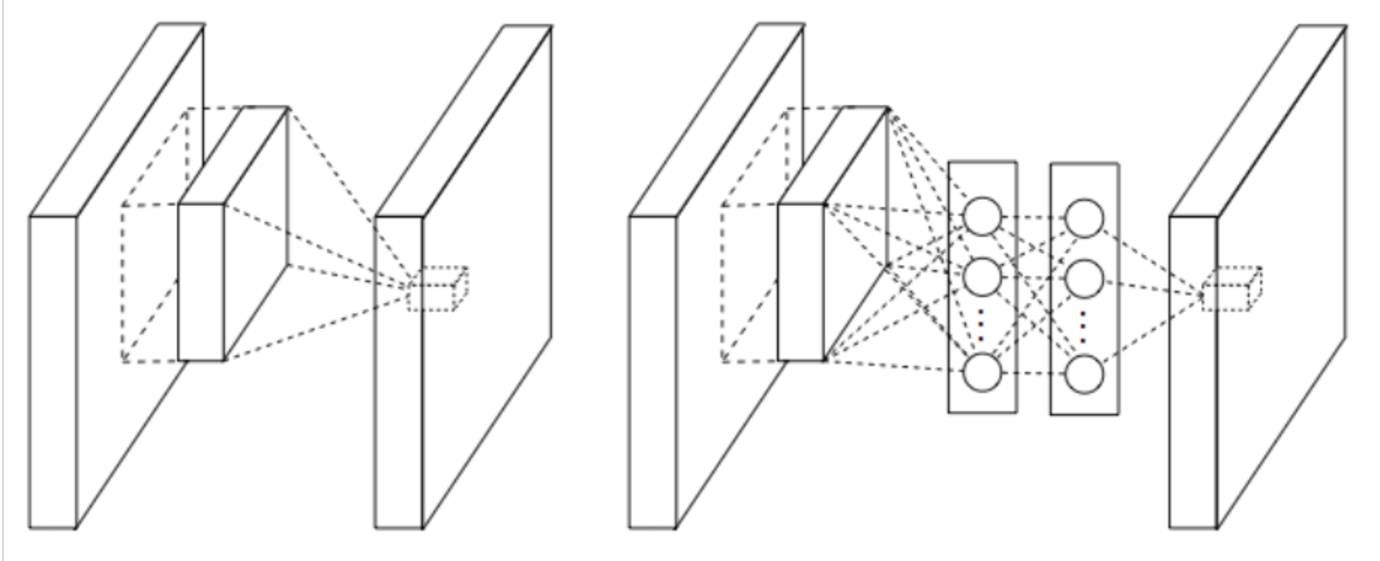
\includegraphics[scale=0.4]{NIN2_1} 
\caption{The ``Network in Network" model from Lin et al. \cite{lin2013network}. The left image shows the operation of a standard CNN convolutional filter, on the right is their approach which replaces the convolutional filter with a miniature neural network.}
  \label{fig:nin}
\end{wrapfigure}
%\end{figure}

Although the title of the original SqueezeNet paper refers to AlexNet (aka “Supervision” \cite{krizhevsky2012imagenet}), the architecture of SqueezeNet has only a passing resemblance to classic CNNs such as AlexNet or VGG \cite{vgg}. Instead it uses a network of repeated ``modules” that are themselves small CNNs; this puts it in the same category as more recent networks such as Google's ``Inception" network (also called ``GoogLeNet”\footnote{The name ``GoogLeNet" is used ambiguously. In PyTorch and elsewhere, it refers to a particular 22-layer version of the Inception network architecture (also known as ``Inception v1”) \cite{szegedy2015going}. But it is also used to refer to Google's winning entry in the 2014 ImageNet competition, which was an \emph{ensemble} of 7 networks, only 6 of which used the Inception v1 design. Details are in the papers describing the multiple incarnations of Inception: \cite{szegedy2015going, ioffe2015batch, szegedy2016rethinking, szegedy2017inception}.}). 

The repeatable building-block design of both Inception and SqueezeNet draw on ideas from the 2013 paper ``Network in Network" from Lin et al \cite{lin2013network}. The authors argue that the convolution filter of a standard CNN provides only a low level of feature abstraction: although it later passes through a non-linear activation function, the filter itself is linear, so represents only what the authors call a ``generalized linear model" of the local input passing through the filter. Better, non-linear function approximators are available, among them are neural networks themselves. The network-in-network approach proposes replacing the linear convolutional filters of a CNN with a ``micro-network", essentially itself a small CNN, see Fig.~\ref{fig:nin}. The micro-network slides over the input in the same manner as a standard convolutional filter, but is better able to represent non-linear features of the input.

Lin et al's micro-networks \cite{lin2013network} make extensive use of 1x1 convolutional filters. These ignore the spatial features captured by larger filters such as 3x3, instead operating only over the channels for a particular point in the input: 1x1 filters essentially perform a per-pixel projection into a lower-dimensional feature space. 

Both SqueezeNet and Google's Inception network employ the network-in-network strategy, making heavy use of 1x1 filters for dimensionality reduction and following a building-block design. The building blocks for SqueezeNet are the Fire modules, Google calls their micro-networks ``Inception modules".











% ``In Convolutional Nets, there is no such thing as "fully-connected layers". There are only convolution layers with 1x1 convolution kernels and a full connection table." - Yann LeCun %https://www.facebook.com/yann.lecun/posts/10152820758292143

% AlexNet: no fixed mirco-level architecture

% VGG: two conv layers followed by pooling layer

% ``Network in Network"- origin of the microarchritectural approach taken by both GoogleNet and Squeezenet.... instead of standard fully-connected convolutional layers, uses ``micro-networks" that are themselves small back-prop networks. 

% - how is this different from adding a layer to a CNN??

% This web article explains Google's Inception module pretty well: https://towardsdatascience.com/a-simple-guide-to-the-versions-of-the-inception-network-7fc52b863202

% My understanding of it is that the Inception module (and the Fire module, I would assume) contains several \textit{parallel} convolutional layers. Moreoever the later versions of the inception modules also purport to improve computations by using some very specific microarchitectures (e.g., replacing a 3x3 layer by a 1x3 followed by a 3x1; instead of having 9 parameters for a 3x3, you have 6, and it's supposed to be as powerful). 

% The ``repeating module" design of both GoogleNet and SqueezeNet closely follows the ideas from the ``Network in Network" paper (\cite{lin2013network}).. this proposes replacing the fully-connected convolutional layers with ``micro-networks" (ie: the modules). The one detail that I have trouble with is how this is any different from just adding layers to the network. The answer seems to rely on the fact of doing convolutions locally rather than globally, but again I fail to see exactly how this differs from the situations in regular CNNs. But... I'll figure it out. 



% - how exactly does a 1x1 convolution kernel accomplish anything at all... related to the ``depth" of the input (visual input is not simply 2D, it has a depth of three channels)

% Xavier: A little late to answer these questions, perhaps,
% but allow me no less. To your first question, what is the 
% difference? I'm guessing it's that having parallel convolutional
% layers means more flexibility and fewer parameters. On a blog
% I was reading regarding Inception modules, they explain that a
% 3x3 convolution = 1x3 convolution followed by a 3x1 convolution
% (or vice-versa). You thus have 6 parameters instead of 9 (smaller,
% fewer computations, less loss? maybe?). I realize this doesn't
% entirely address the question, but it's the best I have for now.
%
% Regarding the second question, from that same blog, I remember 
% reading that 1x1 is supposed to shrink the output. No idea how
% exactly, though. There was also thing about how "7x7" = 5x5 + 1x1.
%


% GoogLeNet: fixed "Inception module" in repeated layers




\section{Proposed Approach}

% \todoOther{proposed layout for this section:\\1. Introductory paragraph or subsection for context.\\2. itemized/point form list of experiments that we ran.\\3 .... followed by prose-form explanations of each point, if necessary...otherwise you need to read a page and a half of prose before you have an idea what's happening}

% here's my attempt at drawing up a list, feel free to correct:

% \Xavier{Good idea. I'll change the prose accordingly.}

% \begin{itemize}
%     \item 1. verifying claim of AlexNet-level accuracy (grid search for both models)
%     \item 2. macroarchitecture experiments (SqueezeNet with one or two fewer layers)
%     \item 3. microarchitecture experiment (adding Batchnorm to Fire module)
% \end{itemize}

% then the prose can be broken up into subsections, one for each item.  \\
% The issues about which database we used and why, and what things we didn't cover can also have their own labeled subsections. This makes it all easier to digest.\\\\

Our project had five objectives:
\begin{description}
    \item[Objective~1] To perform a grid search of learning parameters on both AlexNet and SqueezeNet to guide the remaining objectives.
    \item[Objective~2] To verify the claim that SqueezeNet performs at similar levels of accuracy as AlexNet does using the best parameters obtained in Objective~1 for each model.
    \item[Objective~3] To measure the impact of macroarchitecture modifications to SqueezeNet, namely adding and removing Fire modules.
    \item[Objective~4] To determine the impact of microarchitecture modifications, specifically adding batch normalization layers to SqueezeNet's Fire modules.
    \item[Objective~5] To determine how transfer learning affects learning on CIFAR.
\end{description}

The following sections discuss our choice of dataset, the five objectives, and, finally, elements of the model %and paper
which we did not address.

\subsection{Tools and dataset}

The code for this project, including the models and analyses, were written in Python 3 \cite{python3}. The code for both SqueezeNet and AlexNet was provided by the Torchvision library \cite{torchvision}. Our code also relied heavily on the PyTorch \cite{pytorch} and NumPy libraries \cite{numpy}, and used the SciPy library for statistical testing \cite{scipy} and the Matplotlib library for the figures in the report \cite{Matplotlib}. The models were trained, validated, and tested on Google's Colaboratory \cite{colab}.

% Our project proposes to use CIFAR-10 (Canadian Institute For Advanced
% Research; 10 object classes) \cite{CIFAR-10} in order to 
% (1) to study the impact of learning parameters on SqueezeNet's performance when training from scratch, (2) to reproduce the Iandola et al. \cite{iandola2016squeezenet} results according to which SqueezeNet can be trained to perform at the same level of accuracy as AlexNet, (3) to evaluate the impact of ablating or expanding SqueezeNet by adding or removing Fire modules, and (4) to evaluate
% the impact of adding Batch Normalization layers to SqueezeNet.
% % Transfer learning?
% We chose to work with the uncompressed version of the model and did not use versions of the model which implement bypass connections.
% % Very interesting facts noted below regarding the impact of 
% %compression. Should try to include them.
% The code for the model was provided as part of the Torchvision library \cite{torchvision}. Modifications to the model and analyses used the PyTorch \cite{pytorch} and Numpy libraries \cite{numpy}.

We used the CIFAR-10 dataset (Canadian Institude For Advanced
Research; 10 classes) \cite{CIFAR-10}. This dataset contains $60,000$ images over 10 classes, which we split into a training set ($45,000$ images), a validation set ($5,000$ images), and a test set ($10,000$ images). All images were randomly cropped, resized to $64\times{}64$, and randomly flipped horizontally before each use.

\begin{wraptable}[15]{r}{0.55\textwidth}
%\begin{table}[ht]
    \vspace{-2em}
    \centering
    \makebox[\linewidth]{
        \begin{tabular}{lrrr}
            \toprule
            & & \multicolumn{2}{c}{\textbf{Training time}} \\
            \cline{3-4}\\[-0.7em]
            \textbf{Dataset} & \makecell{\textbf{Size}} & \makecell{\textbf{AlexNet}} & \makecell{\textbf{SqueezeNet}}\\
            \midrule
            ImageNet & 161,075 MB${}^\dagger$ & --- & --- \\
            ImageNet-16 & 923 MB & 1897 s/epoch & 1697 s/epoch \\
            CINIC-10 & 656 MB & 158 s/epoch & 166 s/epoch \\
            CIFAR-100 & 161 MB & 33 s/epoch & 34 s/epoch\\
            CIFAR-10 & 163 MB & 37 s/epoch & 39 s/epoch \\
            \bottomrule
        \end{tabular}
    }
    \parbox{0.55\textwidth}
    {
        \footnotesize ${}^\dagger$ This is actually the size of the dataset for the ILSVRC2014 challenge \cite{ILSVRC14}. It was not readily possible to obtain the size of the ILSVRC2011 dataset which was used for SqueezeNet.
    }
    \caption{Size of the compressed datasets and time elapsed to train each models for one epoch on each dataset using Google Colaboratory.}
    \label{tab:dataset_times}
%\end{table}
\end{wraptable}

%\todo{This paragraph is good... can it be shorter?}
%Shaved off 5 lines...

Many datasets were available for the project: the original ImageNet \cite{imagenet}, ImagetNet variants (i.e., ImageNet-16, ImageNet-32, and ImageNet-64) \cite{imagenet_16_32_64}, CIFAR-10, CIFAR-100 (both from \cite{CIFAR-10}), and CINIC-10 \cite{CINIC-10}. Table~\ref{tab:dataset_times} displays the size of the compressed datasets, as well as the time it took to train each model for a single epoch using Google's Colaboratory GPU processors. Using this table, it is easy to understand why we rejected ImageNet, its variants, and CINIC-10; ImageNet was simply too big, whereas the ImageNet variants and the CINIC-10 training times made them impractical for grid searches. Finally, we also rejected CIFAR-100, since the models' performance over the first few epochs gave us reason to believe that it would take at several dozen epochs to get decent results which also makes this dataset impractical for grid searches. In the end, using CIFAR-10 was simply a pragmatic choice.

% Using CIFAR-10 was a pragmatic choice: we were limited in time and resources, and encountered unexpected difficulties training SqueezeNet. Table~\ref{tab:dataset_times} displays the size of the compressed datasets, as well as the time it took to train each model for a single epoch using Google's Colaboratory CPU processors. We rejected ImageNet due to its size.

% the size of the compressed datasets, as well as the time it took train each model for a single epoch using Google's Colaboratory GPU processors are displayed in Table~\ref{tab:dataset_times}. As shown, even using Colab, ImageNet and its variants were either too big given our resources or too time consuming given the time afforded for the project. As for CINIC-10, we chose CIFAR-10 over it, because of time limitations as well: performing grid searches over a wide variety of parameters like we did would not have been feasible given the CINIC-10 training time. Finally, we did try to use CINIC-100, but, in all of our attempts, both AlexNet and SqueezeNet performed poorly over the first 10 epochs. This suggested that training on a dataset with more classes would most likely require many more epochs, perhaps in the range of 20, 50, or even 100 epochs, in order to a get a representative performance. Again, for these reasons, given our time and resource limitations, CIFAR-10 seemed like the best choice.


% Many datasets were available for the project such as the original ImageNet \cite{imagenet}, ImagetNet variants (i.e., ImageNet-16, ImageNet-32, and ImageNet-64) \cite{imagenet_16_32_64}, CIFAR-10, CIFAR-100 (both from \cite{CIFAR-10}), and CINIC-10 \cite{CINIC-10}. Using CIFAR-10 was a pragmatic choice: we were limited in time and resources, and encountered unexpected difficulties training SqueezeNet. Regarding time and resource limitations, the size of the compressed datasets, as well as the time it took train each model for a single epoch using Google's Colaboratory GPU processors are displayed in Table~\ref{tab:dataset_times}. As shown, even using Colab, ImageNet and its variants were either too big given our resources or too time consuming given the time afforded for the project. As for CINIC-10, we chose CIFAR-10 over it, because of time limitations as well: performing grid searches over a wide variety of parameters like we did would not have been feasible given the CINIC-10 training time. Finally, we did try to use CINIC-100, but, in all of our attempts, both AlexNet and SqueezeNet performed poorly over the first 10 epochs. This suggested that training on a dataset with more classes would most likely require many more epochs, perhaps in the range of 20, 50, or even 100 epochs, in order to a get a representative performance. Again, for these reasons, given our time and resource limitations, CIFAR-10 seemed like the best choice.

% \Xavier{Thank you for your comments. I made changes accordingly. Let me know what you think.}

% \todoOther{Table 1 comments: is ``training time" perhaps better than ``elapsed time?" Elapsed time suggests a total (but I only really noticed because of the typo)} \Xavier{Good point. Changed it.}

% \todoOther{``seconds per epoch" needs context. On what platform?} \Xavier{Another good point. I specified in the paragraph above that we're talking about training time on Colab. It is also mentioned in table caption now and in the first paragraph of this section.}

% \todoOther{Is there a better way to present the 2011 Imagenet details? Either in the caption or elsewhere? Neither the size or time data match the rest of the table. An alternative is to give the size as ``$>$100GB" which makes the size issues clear enough without giving a precise but inaccurate value.} \Xavier{Changed it to MB. 157.3GB * 1024MB/GB = 161075.2MB}

\subsection{Objective 1: AlexNet and SqueezeNet Grid Search}

Our first objective was to find the best parameters for training AlexNet and SqueezeNet. Based on our initial attempts at training SqueezeNet, we figured it out that it would be difficult to train the SqueezeNet model. For instance, one of the first combinations of learning parameters we tried were the ones proposed by Iandola et al. \cite{iandola2016squeezenet} (i.e. learning rate $= 0.1$, momentum $= 0.9$, and weight decay $= 0.0002$), which led to a very poor performance by SqueezeNet ($10.0\%$, chance). We thus decided to obtain the learning parameters more systematically by running a grid search. The parameters and their values are displayed in Table~\ref{tab:grid_parameters}. Both models were trained using all 54 combinations of these parameters and tested using CIFAR-10's test set for each.

% Ended up combining the tables for Aim 3 and 4. Made more sense.
% \Xavier{I combined the following two tables to save space. Feel free to split them up if necessary or if you don't think they should be together. I'm pretty sure the APA would frown on having tables displayed like this.}

\subsection{Objective 2: AlexNet vs SqueezeNet}

Having thoroughly analysed the impact of learning parameters on both models, we then trained them over $50$ epochs using the parameters which had produced the best results in the previous step.


\subsection{Objective 3: Macroablations and macroextensions of SqueezeNet}

We were also interested in the impact of removing and adding Fire modules on SqueezeNet. We believed that some of the issues we faced training SqueezeNet were perhaps due to its size; that, having fewer parameters, there was less room for error in the parameters' values. We expected to find that fewer modules would mean that the model would be that much harder to train, and, conversely, that more modules would make it correspondingly easier to train. In order to evaluate this hypothesis, we ran four experiments. In the first two, we created two modified versions of SqueezeNet from which one and two Fire modules were removed from the end. The last remaining Fire module's parameters were also adapted to fit with the ``classifier" portion of the model. For the third and fourth experiments, we created two versions of the model with one and two extra Fire modules, respectively. Each experiment then consisted of running a grid search identical to the one in Objective 1 with the exception that the batch size was fixed at $64$ and weight decay, $0$. The parameters are displayed in Table~\ref{tab:grid_parameters}.

%Transfer learning? 
%Indeed, I'm sad there was none, especially after sufferring through assignment 3, and breaking into subsections accordingly
% Xavier: There could be, if I find the time and something to say.
%   Honestly, it feels like we *should* mention it. All of these
%   issues were facing largely go away when using transfer
%   learning... I just don't really have time or want to do a
%   grid search on SqueezeNet. If anyone does, the code already
%   exists: we could easily run a transfer learning experiment
%   with both AlexNet and SqueezeNet on CIFAR-10 (or EMNIST).

% \Xavier{I combined the following two tables to save space. Feel free to split them up if necessary or if you don't think they should be together. I'm pretty sure the APA would frown on having tables displayed like this, but this is a term paper...}

% \todoOther{looks fine. The first column is the same in both tables, so it could be a single three-column table (with ``Objective 2" and ``Objective 3" columns)}

% \Xavier{Good point. I'll leave it as is for now, but feel free to change it. I think it'll work either way. \textbf{If you do change it, please make sure to update the \textbackslash{}ref in the text.} Thank you! }

\begin{table}[hb]
    % \centering
    % \parbox{.45\linewidth}{
        \centering    
        \begin{tabular}{lllll}
            \toprule
            \textbf{Parameter} & \textbf{Objective 1} & \textbf{Objective 3} & \textbf{Objective 4} & \textbf{Objective 5}\\
            \midrule
            Batch size & 64, 512, 1024 & 64 & 64 & 64\\
            Learning rate & 0.05, 0.01, 0.001 & 0.05, 0.01, 0.001 & 0.2, 0.1, 0.05, 0.01, 0.001 & 0.05, 0.01, 0.001\\
            Momentum & 0.9, 0.5, 0.1 & 0.9, 0.5, 0.1 & 0.9 0.5, 0.1 & 0.9 0.5, 0.1\\
            Weight decay & 0, 0.002 & 0 & 0 & 0\\
            \bottomrule
        \end{tabular}
        \caption{Grid search parameters for Objectives~1, 3, and 4.}
        \label{tab:grid_parameters}
    % }
    % \hspace{2em}
    % %\hfill
    % \parbox{.45\linewidth}{
    %     \centering    
    %     \begin{tabular}{ll}
    %         \toprule
    %         \textbf{Parameter} & \textbf{Values} \\
    %         \midrule
    %         Batch size & 64\\
    %         Learning rate & 0.2, 0.1, 0.05, 0.01, 0.001\\
    %         Momentum & 0.9, 0.5, 0.1\\
    %         Weight decay & 0\\
    %         \bottomrule
    %     \end{tabular}
    %     \caption{Grid search parameters for Objective~4. These were applied to various modified versions of SqueezeNet.}
    %     \label{tab:batch_norm_parameters}
    % }
\end{table}

\subsection{Objective 4: Batch Normalization layers}

One obvious solution to the difficulties we were facing with training SqueezeNet was to add batch normalization layers. Following Ioffe and Szegedy's suggestion to place batch normalization layers before non-linearies such as ReLUs \cite{ioffe2015batch} and taking inspiration from the VGG-19 architecture \cite{vgg}, we modified the microstructure of the Fire modules by inserting a batch normalization layer between first convolution layer and the first layer of ReLUs. The parameters used for this experiment are displayed in Table~\ref{tab:grid_parameters}. We expected that adding batch normalization layers would greatly improve the ability of the network to learn and that it would be able to handle larger learning rates.


\subsection{Objective 5: Transfer learning}

One other way to improve a model's ability to learn is to use transfer learning. That is to say that we can use the parameter values found by Iandola et al. on ImageNet as starting points, then finetune the network parameters on CIFAR-10 data. Transfer learning is an effective and commonly used technique, particularly in domains such as medical imaging where labelled data is scarce \cite{pan2010survey, huh2016makes}.

% \todo{Add justification for why transfer learning makes sense \textbf{in the context of the training difficulties we're having.}}

% \todoOther{One option may be to talk about the results of Objective 2. Though SqueezeNet is out-performing AlexNet in all the runs, neither has been able to reach the performance recorded in the table so far. This highlights the importance of initial weights.}

% \todoOther{This sounds good. It also makes sense to look at transfer learning for its own sake, since this is how it will often be used in the field; in medical imaging applications for example, transfer learning is pretty much always used, since the amount of labelled data is small.}


% \todo{\textbf{\underline{Will need to mention that seed was set only once, before running experiments!}}\\Unfortunately, this means that there is no easy way for us to reproduce the results...}


\subsection{Unaddressed issues}



% \Xavier{Bypass connections could have been an interesting alternative to Batch Normalization (I believe Gordon actually mentioned that on Slack at some point). We could therefore consider it at limitation of our approach not to have looked at that. One other limitation is that the analyses did not keep track of the seed. I only realized much later that that may be of importance.}
% \todo{I don't remember saying that... that makes me sound smarter than I probably am. Bypass seems  to be a way around the large amount of dimensionality reduction in the modules, I'm not sure if that relates to batchnorm or not. I'd be open to a ``limitations" section, but it needs to a single sentence, preferably at the end of the paper. We should focus on writing now.}


Our report does not consider model compression or the addition of bypass connections. Bypass is mentioned only in a single section of the paper and is not part of the central results, and is not present in the PyTorch implementation of SqueezeNet. This was left out in the interests of time. 

Concerning model compression, standard SqueezeNet has a size of 4.8MB. The ``$<$0.5 MB model size" claim in the paper refers to the size of SqueezeNet after undergoing a compression technique called ``deep compression," involving network pruning, quantizing weights to lower bit depths, Huffman coding, and other techniques, detailed in Han el al. \cite{han2015deep}. We have not considered the compressed model size of SqueezeNet for a number of reasons:
\begin{itemize}
\item Neither SqueezeNet nor AlexNet suffer any accuracy loss when using deep compression. This is not a technique particular to SqueezeNet or that favours either model.
\item Deep compression moves the sizes of the models closer together: compressed SqueezeNet is $\sim$14.5 times smaller than compressed AlexNet, substantially less than the 50x difference between uncompressed models given in the title of the SqueezeNet paper.
\item The compression details are not part of the SqueezeNet paper. 
\end{itemize}
The authors' sole point about model size seems to be that, although SqueezeNet is small, it can still be compressed further without loss of accuracy, to a size small enough to consider printing on a chip. This is not without interest, but arguably speaks more to the power of the deep compression technique itself, which has been applied across different models with similar results. 





%\todo{Say something about that here. There's some interesting prose below; good job to whomever wrote that. May be useful here.}

%I'm still open to hearing why this is a problem, but we need to finish. 

%\textbf{Bypass connections.} In our model we have not utilized the bypass connection, since using a simple bypass impose the limitation to the design due to the need of according between the number of input and output channels and the complex output increase the number of parameters without improving the accuracy of the model \cite{iandola2016squeezenet}. \todo{Could be consider as the reason that we have not used the bypass in the model. but you can remove it, if you want.It is based on the original paper}
%\todoOther{I'm just trying to understand what claim is being made... this is a restriction on the architecture: only modules with matching values can be connected. It's not clear to me how that explains why we're not investigating it.}





% \todo{``Reproduce the results reported in the paper by running the code provided by the authors."}

% %\todo{``Then you will try to modify the model and perform ablation studies to understand the model’s robustness and evaluate the importance of the various model components. You can also try to improve the model based on your experiments. You should do a thorough analysis of the model through an extensive set of experiments. At a minimum, in this track you should use the authors code to reproduce a non-trivial subset of their results and explore how the model performs after you make minor modifications (e.g., changes to hyperparameters). An outstanding project in this track would perform very a detailed ablation study and/or implement significant/meaningful extensions of the model."}

% %Preprocessing? Typical preprocessing step is to normalize input by mean and standard deviation of the data.... in cases where this is expensive to do a common step is to use the mean and std. dev. of imagenet data, typically this is better than not normalizing at all.\\\\


% %Transfer learning
% %- note that there are in general two distinct kinds of transfer learning:
% %- ``finetuning": start with a pre-trained model and continue training with a new dataset, essentially retraining the entire model
% %- ``feature extraction", start with a pre-trained model, but training on the new dataset changes the weights in the final layer only (use ``\texttt{requires\_grad = False}")\\\\\

% Possible experiments? 

% - should we leave the ``Fire Modules" as-is and only experiment with the macroarchitecture? 

% what happens if we swap out ``fire modules" for Google's ``Inception" module and keep everything else the same? How do they differ at the micro- and macro-level?

% \textit{Other possible experiment: add another fire module layer or classifier module.}
% \begin{enumerate}
%     \item It could be interesting to evaluate the importance of adding/remove a "layer" (especially since the model is essentially a series of "fire" modules/layers).
%         \begin{enumerate}
%             \item Removed the last Fire module. It had little to no impact on performance. I will need to verify the learning parameters and compare it with the best SqueezeNet we got.
%             \begin{enumerate}
%                 \item May be interesting to see how it performs on a different dataset, namely CINFAR-100 with 20 classes (coarse classes). It is possible that the final module isn't necessary with only 10 classes, because of the number of classes, but that with a higher number of classes, it would become necessary.
%                 \item Could try removing layers until it can't perform on 20 or 100 classes, then see if it can still work with 10?
%             \end{enumerate}
%             \item 
%         \end{enumerate}
%     \item VGG has a "classifier" at the end (a series of linear layers with BatchNorm and DropOut layers). SqueezeNet doesn't include those, saying that they aren't necessary (Nin; Lin et al., 2013).
% \end{enumerate}

% - hyperparameters?

%- Note that a *trained* version of SqueezeNet is availably in PyTorch:\\\texttt{net = torchmodels.SqueezeNet1\_1(pretrained=True)}\\ So it should be easy to reproduce the reported ImageNet accuracy for SqueezeNet, although this isn't an ``experiment," so shouldn't be a priority. BUT, since a trained version is available, one possible experiment is to see how good the model is at transfer learning compared to transfer learning with VGG, AlexNet or GoogleNet. This is some sort of measure of the robustness of the model. This is also something we can do in a tractable amount of time. 

% - what's the training time? \todo{Will need to compare training time on ImageNet-16 and CIFAR-10. CIFAR-10 undoubtedly takes significantly less time. ImageNet cannot realistically be used given the amount of time we have and the fact that we want to run experiments.} \textit{Note: the training time is very similar between the models and is actually a little smaller for AlexNet than SqueezeNet [On CINIC-10, 158s/epoch vs 166s/epoch].}
% % This is a temporary table, just a place for me to write the training times.


% \todo{Need to mention that we had to resize the CIFAR images to 64x64.} They are originally 32x32 images, but we resized them to 64x64 using textbf{nearest neighbor}. We chose this method, because it leaves the original pixel information unaffected.

% % Tests to run:

% %     \todo{... note here that the network most similar to SqueezeNet is actually ``GoogLeNet" rather than AlexNet, something I'm already drawing up related work notes on. Is there room / time to include GoogLeNet in any comparisons?\\ And if transfer learning tests are cheap, we should consider including VGG as well, since AlexNet, VGG and GoogLeNet all have quite different architectures.}
% % \begin{itemize}
% %     \item Comparison AlexNet and SqueezeNet on ImageNet/CIFAR-10/CIFAR-100/CINIC-10/etc.
% %     \item Transfer learning of SqueezeNet vs AlexNet on Extended MNIST
% %     \item hyper-parameter tuning
% %     \item ``ablation study"
    
% % \end{itemize}



\section{Results and Discussion}

% I don't think this is necessary
%In this section, we review the results for each aim, before moving on to a general discussion of our results.

\subsection{Objective 1: AlexNet and SqueezeNet Grid Search}

The results of our grid search on the impact of learning parameters on SqueezeNet and AlexNet are presented in Table~\ref{tab:alex_squeeze_grid}. There are three things to note. First, as noted previously, the learning parameters recommended to train SqueezeNet on ImageNet \cite{iandola2016squeezenet}, namely $learning rate = 0.01$, $momentum = 0.9$, and $weight decay = 0.0002$, lead to chance-level accuracy ($10\%$) on CIFAR-10 using a batch size of $64$ and mild accuracy using larger batch sizes ($29.76\%$ for a batch size of $512$ and $19.28\%$ for a batch size of $1024$). Second, the best parameters for both AlexNet and SqueezeNet within our search space and their corresponding performance are displayed in Table~\ref{tab:best_alex_squeeze}. These parameters were used in our second objective. The third and last thing to note is that both models performed best with a batch size of $64$ and that weight decay, for a batch size of $64$, had little-to-no effect. We therefore chose to fix those parameters to $64$ and $0$, respectively, in order to reduce the search space for our other grid searches.

\begin{table}[ht]
    \centering
    \begin{tabular}{lrrrrr}
        \toprule
        \textbf{Model} & \textbf{Batch size} & \textbf{Learning rate} & \textbf{Momentum} & \textbf{Weight decay} & \textbf{Accuracy} \\
        \midrule
        AlexNet & 64 & 0.01 & 0.9 & 0 & 40.74\\
        SqueezeNet & 64 & 0.001 & 0.9 & 0.0002 & 40.04\\
        \bottomrule
    \end{tabular}
    \caption{The parameters within our search space which led to the highest performances for both models and the corresponding accuracy on the test set. The full results table, Table~\ref{tab:alex_squeeze_grid}, can be found in the Appendix.}
    \label{tab:best_alex_squeeze}
\end{table}


\subsection{Objective 2: AlexNet vs SqueezeNet}

Figure~\ref{fig:AlexNet_vs_SqueezeNet} compares the performances of AlexNet and SqueezeNet when using optimal parameters. The plots on the left represent runs which used the parameters described in Table~\ref{tab:best_alex_squeeze}. These runs also used a step scheduler which reduced the learning rate by a factor of 10 every 10 epochs. The plot on the right displays a run using a different set of parameters: AlexNet was trained using a batch size of $64$, a learning rate of $0.0125$, a momentum of $0.5$, and a weight decay of $0$, and SqueezeNet was trained using a batch size of $64$, a learning rate of $0.01$, a momentum of $0.1$, and a weight decay of $0$. This run also used an adaptive scheduler \cite{optim} rather than a step scheduler; the adaptive scheduler reduced the learning rate by half if the model's validation loss had not decreased over the last three epochs. We present this run here because it led to the highest performances by both models while showing that SqueezeNet is able to match AlexNet's high performance.

%\todo{I don't known what a ``chance run" is}

%\todo{Does ``right" here mean correct, or the parameters used for the plot on the right in the figure?}
% Fixed. Thank you.


% This should probably be in the discussion instead.
% There are two takeaways. First, given a good set of parameters, it appears that SqueezeNet can match and even outperform AlexNet, even when the latter performs at its best. This confirms the findings by Iandola et al. \cite{iandola2016squeezenet} on CIFAR-10 and achieves our second objective.

% The second takeaway, however, is that initial weights matter. The plots on the left were created from three sequential runs where the seed was not reset. As the plots show, the model's performance can vary between runs. In fact, during the best of the three runs, AlexNet achieved an accuracy of $22.75\%$ whereas SqueezeNet achieved $33.40\%$. Both of these are far below their respective $40.74\%$ and $40.04\%$ from our grid search.

% I scaled this down slightly for space considerations
\begin{figure}[ht]
% \begin{wrapfigure}{r}{0.6\textwidth}
    \centering
    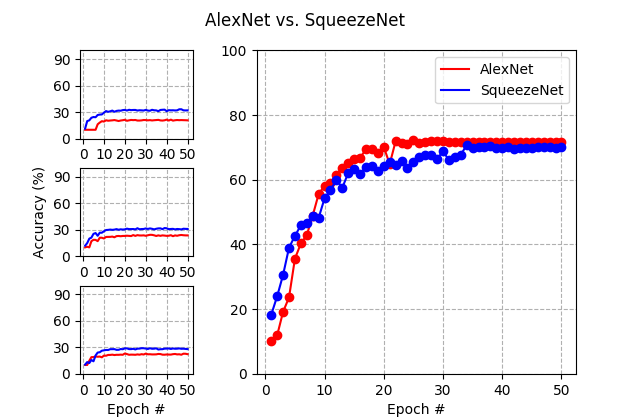
\includegraphics[scale=0.7]{aim2_vs.png}
    \caption{AlexNet vs. SqueezeNet. This figure highlights both the fact that SqueezeNet can match AlexNet's performance and even outperform it, but also that initial weights appear to matter enormously when training these models. For the three plots on the left, the parameters used were those reported in Table~\ref{tab:best_alex_squeeze}. For the large plot on the right, both models were trained using an alternative set of parameters and using an adaptive scheduler, rather than a step scheduler.}
    \label{fig:AlexNet_vs_SqueezeNet}
% \end{wrapfigure}
\end{figure}

\subsection{Objective 3: Macroablations and macroextensions of SqueezeNet}


We had hypothesized that some of our issues with training SqueezeNet came, perhaps, from its size: with fewer parameters, there would be less room for error. This was motivated, namely, by prior experience with the VGG-19 model on a previous assignment. The results of our grid searches are presented in Table~\ref{tab:ablation_expansion_grid}. In order to determine whether model size did have an impact, for each condition in our grid searches, we calculated a relative test accuracy for each experimental model. More specifically, we subtracted the experimental model's performance by that of the original, unmodified SqueezeNet for that condition. These relative test accuracies are displayed in Figure~\ref{fig:objective3}. Though there does appear to be effect, we found a correlation \cite{crowder2017analysis} of $r=-.1972$ which was not statistically significant, $p=0.2489$.

\subsection{Objective 4: Batch normalization layers}

Our fourth objective was to evaluate the impact that adding batch normalization layers to the Fire modules would have on model performance. The results of the grid search are presented in Table~\ref{tab:batchnorm_grid}. Using a repeated measures t-test \cite{crowder2017analysis}, we confirmed that the new model with added batch normalization layers performed significantly better than the original model; $t = 3.14$ (repeated measure), $p < .05$.


% \begin{figure}[htb]

\begin{wrapfigure}[11]{r}{0.55\textwidth}
    \vspace{-5.5em}
    \centering
    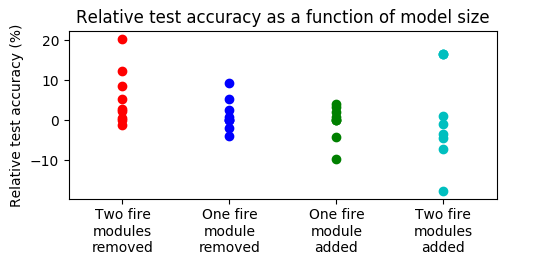
\includegraphics[scale=0.7]{aim3_corr.png}
    \caption{The impact of macroablations and macroexpansions on SqueezeNet's performance after 10 epochs. All relative test accuracies were calculated by subtracting the modified model accuracy with the unmodified SqueezeNet's accuracy under the same conditions.}
    \label{fig:objective3}
\end{wrapfigure}
% \end{figure}


% Make figure to match the one for objective #2, but with batchnorm? For contrast. Use green for batchnorm.p

% \todo{not sure what your results are here, but here's an extra sentence for the experiments I ran:}

% \Xavier{ I'm not sure how to include your experiments. They don't really fit with the overall "story" of: we tried it this way because  that's what the original paper suggests and that's what works  with VGG. Also, since you didn't find anything interesting, I'm not sure what to do or say about it and feel like it takes  away from the main (and really cool) point that BatchNorm layers, when used in that way, make a huge difference.}

% \todo{That's fine... there IS a positive finding (yours).. VGG has a classic CNN architecture, which SqueezeNet does not, so I don't see any great contradiction in finding that it doesn't work when used outside of the module. I don't think we should spend too much time debating it. }

% \Xavier{ I would argue that VGG's architecture is more similar to SqueezeNet than you say. Really, the big difference is that SqueezeNet has convolutional layers that are split. Otherwise, they look pretty similar. In any case, if it's all the same to you, I would prefer to keep it to what I found for now. If you find something to add to the discussion with your results (once that's written), then sure.
% }

% \todo{I'm much happier to leave it out than continue debating it, that's for sure.}

% \Xavier{Unrelated thought: SqueezeNet with BatchNorm performs so well... it may just be America's Next Top Model! Hahaha}

%We also ran numerous experiments leaving the Fire modules unchanged, and adding batchnorm layers to different parts of the network: before or after ReLU, before some or all Maxpooling layers, or after every Fire module. In all cases we found that adding batchnorm layers had only a minor effect on performance.


\subsection{Objective 5: Transfer learning}

%\todo{this is nice and short! Should it say ``as expected" instead of "of note"? } Xavier: Yes, good suggestion, thank you!

The results for transfer learning on CIFAR-10 using the model parameters from ImageNet are in Table~\ref{tab:transfer_cifar_grid}. As expected, the model performed significantly better using the ImageNet parameters than random parameter values; $t=2.33$ (repeated measures), $p < .05$.

\subsection{General discussion}

% \Xavier{I realize that I am repeating myself below. I'm still working out exactly what I want to say. Suggestions are welcome.}

% \todo{Initial comments on first reading: could emphasize the postive result, and spend much less space discussing the results that are far less certain. I'm not really done reading yet though. Can also completely skip the first few sentences that repeat the results.}


% Our project began with four objectives: to find the best parameters for both SqueezeNet and AlexNet, to use those parameters to verify the claim that SqueezeNet could perform just as well as AlexNet, to measure the impact of macroablations and macroexpansions on the model, to determine whether adding Batch Normalization layers to SqueezeNet could improve its to learn, and, lastly, to evaluate the gains from using pre-training.

% We ran a grid search in order to find the best parameters for training AlexNet and SqueezeNet. We then went on to use the best of those parameters to compare the models' performances, but were surprised to find that the models performed significantly more poorly than they had during grid search. We investigated and discovered that this was likely due to the random initialization of the models' weights before training. More specifically, it appears that SqueezeNet (as well as AlexNet, to some extent) has an irregular optimization landscape with many local minima, but few of which are significant. During training, the model is therefore likely to be pulled toward a shallow minima rather than a deeper one which ultimately limits the model's performance significantly. In short, the model's initial weights, that is the position of the model's parameters in the optimization landscape, appears to be very important in the model's max performance.

Using a grid search, we found the combinations of parameters under which AlexNet and SqueezeNet performed best after ten epochs. Using those to compare the models' performances over 50 epochs, we came to two conclusions.

The first is that, given a good set of parameters, SqueezeNet is indeed able to match or even outperform AlexNet, even when the latter is trained using its best set of parameters (see Figure~\ref{fig:AlexNet_vs_SqueezeNet}).

The second is that parameter initialization matters. That is to say that we were surprised to find that the models performed significantly more poorly when trained on 50 epochs than they had during grid search. After investigating, we discovered that the random number generator seed was only set at the beginning of the experiment, meaning that the models in the searches were initialized with different parameter values. That parameter initialization has such a strong impact on performance suggests that SqueezeNet may have an irregular optimization landscape in which the starting position is very important. One can imagine, for example, that there may be many local minima, most of which are shallow, with a few deep minima which greatly increase the model's performance. 

%\todo{Do you understand what I mean by "shallow" and "deep" minima? Should I find a different way of explaining this?}

% These results suggest that SqueezeNet (and as AlexNet, to an extent) has an irregular optimization landscape with many local minima, but few of which are significant. During training, the model is therefore likely to be pulled toward a shallow minima rather than a deeper one which ultimately limits the model's performance significantly. In short, the model's initial weights, that is the position of the model's parameters in the optimization landscape, appears to be very important in the model's max performance.


% There are two takeaways. First, given a good set of parameters, it appears that SqueezeNet can match and even outperform AlexNet, even when the latter performs at its best. This confirms the findings by Iandola et al. \cite{iandola2016squeezenet} on CIFAR-10 and achieves our second objective.

% The second takeaway, however, is that initial weights matter. The plots on the left were created from three sequential runs where the seed was not reset. As the plots show, the model's performance can vary between runs. In fact, during the best of the three runs, AlexNet achieved an accuracy of $22.75\%$ whereas SqueezeNet achieved $33.40\%$. Both of these are far below their respective $40.74\%$ and $40.04\%$ from our grid search.


We hypothesized that the irregular shape of the optimization space might be due to the fact that SqueezeNet is smaller: it has fewer parameters and therefore less room for error. The results from Objective 3, however, suggest otherwise. Instead, these results suggest that the issue may be one of propagation: loss is more easily back propagated through the smaller models which are therefore able to improve more quickly. This is consistent with results from Bjorck et al. \cite{UnderstandingBatchNorm} who reported that large gradient updates were more likely to result in diverging losses in deeper models.
This also fits with the common adage in Machine Learning: ``Deeper neural networks are more difficult to train" \cite{resnet}.

Given the difficulties we faced with training SqueezeNet, one obvious solution was to add batch normalization layers. Adding batch normalization layers significantly increased SqueezeNet's ability to learn, as well as the speed at which it learned. These results are in line with previous studies on the impact of implementing batch normalization layers \cite{UnderstandingBatchNorm}.

% \todo{I think the next paragraph is good, but could be much shorter, like two sentences} \Xavier{I will see what I can do.}

This begs the question: Why, then, did the authors not include batch normalization layers in the original model? We believe that it is possible that the authors did not know about them or learned about them too late. The Ioffe et al. \cite{ioffe2015batch} paper came out only a year before the Iandola et al. \cite{iandola2016squeezenet} paper was first submitted. The other possibility is that the authors underestimated the importance of batch normalization layers. We found that a second version of SqueezeNet, SqueezeNet 1.1 \cite{squeezenet_1_1_maybe}, does not implement batch normalization either and although SqueezeNext \cite{SqueezeNext}, the spiritual successor to SqueezeNet, does implement them, the paper only mentions batch normalization once, in passing. Whatever the case may be, it is worth mentioning that adding batch normalization layers in the way that we have only adds $1673$ parameters to the model, an increase of $0.13\%$ in the number of parameters. The issue is therefore not one of size.

Finally, we used transfer learning to train SqueezeNet on CIFAR-10. As expected, we found that the model performed significantly better over a wide range of learning parameters. This again highlights the importance of initial parameter values.

\section{Conclusion}

In conclusion, initial parameter values matter and starting with a pre-trained model makes training significantly easier. If using a pre-trained model is not an option, we recommend using batch normalization layers. Though they do increase the number of parameters in the model, we believe that they are a worthy addition, since they make the model much easier to use. After all, ``size isn't everything, it's what you (can) do with it that counts.''

% We considered two possibilities. First, it was possible that they authors did know about Batch Normalization layers, and, second, that they underestimated their impact. Regarding the first possibility, it should be noted that the original paper by Ioffe et al. \cite{ioffe2015batch} came out in March 2, 2015, whereas the Iandola et al. paper was first submitted February 24th, 2016. It is possible that most of the work on developing the first version of SqueezeNet had already been done by the time the Ioffe et al. paper was submitted and that, by mid- and late-2015, the authors were focusing on preparing the paper for publication. It is also likely that the importance of Batch Normalization layers was only realized over several months or years after the paper's publication and that, again, by that point, most of the work on SqueezeNet had already been completed. In fact, we note that a second version of SqueezeNet, which appears to have been created in 2017 \cite{squeezenet_1_1_maybe}, did not use Batch Normalization either, but that the spiritual successor to SqueezeNet, namely SqueezeNext, does \cite{SqueezeNext}. That being said, in support of the second possibility, it should be noted that Batch Normalization layers are only mentioned once in the paper, in passing. This, on the contrary, suggests the the authors underestimate their impact on their model. Whichever the case may be, it is worth mentioning that adding Batch Normalization layers in the way that we have only adds $1673$ parameters to the model (i.e., an increase of $0.13\%$). The issue is therefore not one of size.


% \Xavier{Tentative conclusion: In conclusion, though they do increase the number of parameters in the model, we believe that the authors should consider adding Batch Normalization layers to the SqueezeNet 1.0 official version. After all, "size isn't everything, it's what you (can) do with it that counts."}

% \begin{itemize}
%     \item We performed a grid search on SqueezeNet and AlexNet.
%     \item We used that to show that SqueezeNet can perform as well if not better than AlexNet.
%     \item A lot of variability in the training parameters. Non-repeatability. Initial parameter values seem to matter a lot. Irregular optimization space? (Probably not "irregular" in that most models probably are like that, but in that it has an irregular, non-convex shape which makes it harder to "explore").
%     \item Surprising result: more isn't better (size isn't everything).
%     \item Awesome result: Batch norm improves performance significantly. \textbf{Why doesn't SqueezeNet use this?} \Xavier{SqueezeNet 1.1 still doesn't use it, but SqueezeNext does.}
%     \item Transfer learning?
% \end{itemize}

% \todo{Result \#1: Parameters proposed in paper do not work for CIFAR-10.} This isn't groundbreaking, but is worth mentioning either here or elsewhere.

% why doesn't SqueezeNet use batchnorm?




% \todo{Talk about Batch Normalization; make the case that:\\
% (1) It is easy to implement.\\
% (2) Only adds ~1600 parameters [will get exact count]\\
% (3) Maybe wasn't added because it was new back then (oversight)\\
% {[3a]} Should check whether 1.1 version and SqueezeNext include Batch Normalization layers.\\ XXXX it's not in 1.1, you can see this code in our Colab. It IS in SqueezeNext, although they barely mention it, they don't sell it as a central feature. \Xavier{Very good point! Thank you!}
% (4) Authors may have underestimated it's strength.\\
% }

\section*{Statement of Contributions}
%\todo{Draft, feel free to alter your own contributions accordingly}

All members contributed equally to the report and to the direction of the project. Most of the programming was handled by Xavier. Everyone contributed to running the experiments (Colab requires frequent interaction).

\bibliography{biblio}
\clearpage

\section*{Appendix}
\setcounter{table}{0}
\renewcommand{\thetable}{A\arabic{table}}

% \todoOther{For the tables, are all results equally interesting, or are there some ``good" results that can be bolded to stand out? I can't tell just by quickly looking.}

% \Xavier{First, I would say that I don't think it would be appropriate to embolden parts of a table. There may be sections which we don't find important but which a reader who has different ideas and hypotheses than we do would find important. Second, many sections of these tables are interesting. Which ones are interesting depends on what we're talking about. Some of the sections overlap. This would make it hard to choose which sections to overlap/highlight. Finally, I would say that that's what the text is for. If you want to know which results were interesting, you have to read the text. Without the text, you wouldn't be able to know why the results are important.}

% \todoOther{Okay, good... I had only skimmed the text so wasn't sure if there was a ``best hyperparameters" result with the best performance, typically bolded in most ML papers I've read in the past few weeks. What are the units for the last two columns in the first table? percent accuracy?}

% \Xavier{Yes, percent accuracy. I added it. Thank you!}

\begin{longtable}[c]{llllll}
    % \centering
    % \makebox[\textwidth][c]{
%%%%%%%%%%%%%%%%%%%%%%%%%%%%%%%%%%%%%%%%%%%%%%%%%%%%%%%%%%%%%%%%%%%%%%%%%%%%%%%%%%%
% DO NOT EDIT. This table was generated automatically. The following latex code   %
% may be replaced without warning or consideration for modificaitons made.        %
%%%%%%%%%%%%%%%%%%%%%%%%%%%%%%%%%%%%%%%%%%%%%%%%%%%%%%%%%%%%%%%%%%%%%%%%%%%%%%%%%%%
% \begin{tabular}{cccccc}
  \toprule
  \textbf{Batch size} & \textbf{Learning rate} & \textbf{Momentum} & \textbf{Weight decay} & \makecell{\textbf{AlexNet}\\\textbf{accuracy (\%)}} & \makecell{\textbf{SqueezeNet}\\\textbf{accuracy (\%)}} \\
  \midrule
    \multirow{18}{*}{64} & \multirow{6}{*}{0.05} & \multirow{2}{*}{0.9} & 0 & 10.0 & nan \\
     &  &  & 0.0002 & 10.0 & nan \\
    \cline{3-6}
     &  & \multirow{2}{*}{0.5} & 0 & 10.0 & nan \\
     &  &  & 0.0002 & 19.92 & nan \\
    \cline{3-6}
     &  & \multirow{2}{*}{0.1} & 0 & 28.85 & nan \\
     &  &  & 0.0002 & 29.53 & nan \\
    \cline{2-6}
     & \multirow{6}{*}{0.01} & \multirow{2}{*}{0.9} & 0 & 40.74 & 27.69 \\
     &  &  & 0.0002 & 22.57 & 10.0 \\
    \cline{3-6}
     &  & \multirow{2}{*}{0.5} & 0 & 31.96 & 32.49 \\
     &  &  & 0.0002 & 27.77 & 33.35 \\
    \cline{3-6}
     &  & \multirow{2}{*}{0.1} & 0 & 20.46 & 35.21 \\
     &  &  & 0.0002 & 24.78 & 35.23 \\
    \cline{2-6}
     & \multirow{6}{*}{0.001} & \multirow{2}{*}{0.9} & 0 & 22.67 & 37.49 \\
     &  &  & 0.0002 & 23.25 & 40.04 \\
    \cline{3-6}
     &  & \multirow{2}{*}{0.5} & 0 & 10.0 & 33.04 \\
     &  &  & 0.0002 & 11.78 & 33.47 \\
    \cline{3-6}
     &  & \multirow{2}{*}{0.1} & 0 & 10.03 & 30.73 \\
     &  &  & 0.0002 & 10.02 & 29.06 \\
    \cline{1-6}
    \multirow{18}{*}{512} & \multirow{6}{*}{0.05} & \multirow{2}{*}{0.9} & 0 & nan & nan \\
     &  &  & 0.0002 & 10.0 & nan \\
    \cline{3-6}
     &  & \multirow{2}{*}{0.5} & 0 & 10.0 & nan \\
     &  &  & 0.0002 & 20.76 & nan \\
    \cline{3-6}
     &  & \multirow{2}{*}{0.1} & 0 & 10.0 & 10.0 \\
     &  &  & 0.0002 & 18.47 & 10.0 \\
    \cline{2-6}
     & \multirow{6}{*}{0.01} & \multirow{2}{*}{0.9} & 0 & 10.0 & 24.24 \\
     &  &  & 0.0002 & 19.26 & 29.76 \\
    \cline{3-6}
     &  & \multirow{2}{*}{0.5} & 0 & 10.0 & 24.85 \\
     &  &  & 0.0002 & 10.04 & 24.25 \\
    \cline{3-6}
     &  & \multirow{2}{*}{0.1} & 0 & 10.0 & 24.31 \\
     &  &  & 0.0002 & 9.96 & 22.39 \\
    \cline{2-6}
     & \multirow{6}{*}{0.001} & \multirow{2}{*}{0.9} & 0 & 10.2 & 28.8 \\
     &  &  & 0.0002 & 10.78 & 20.11 \\
    \cline{3-6}
     &  & \multirow{2}{*}{0.5} & 0 & 10.0 & 20.77 \\
     &  &  & 0.0002 & 10.0 & 14.53 \\
    \cline{3-6}
     &  & \multirow{2}{*}{0.1} & 0 & 10.0 & 18.37 \\
     &  &  & 0.0002 & 10.0 & 19.67 \\
    \cline{1-6}
    \multirow{18}{*}{1024} & \multirow{6}{*}{0.05} & \multirow{2}{*}{0.9} & 0 & 19.77 & nan \\
     &  &  & 0.0002 & nan & nan \\
    \cline{3-6}
     &  & \multirow{2}{*}{0.5} & 0 & 10.0 & 10.0 \\
     &  &  & 0.0002 & 10.0 & nan \\
    \cline{3-6}
     &  & \multirow{2}{*}{0.1} & 0 & 10.58 & 10.0 \\
     &  &  & 0.0002 & 10.0 & 10.0 \\
    \cline{2-6}
     & \multirow{6}{*}{0.01} & \multirow{2}{*}{0.9} & 0 & 10.0 & 15.84 \\
     &  &  & 0.0002 & 10.0 & 19.28 \\
    \cline{3-6}
     &  & \multirow{2}{*}{0.5} & 0 & 10.0 & 17.72 \\
     &  &  & 0.0002 & 10.0 & 17.47 \\
    \cline{3-6}
     &  & \multirow{2}{*}{0.1} & 0 & 11.59 & 12.38 \\
     &  &  & 0.0002 & 10.0 & 19.79 \\
    \pagebreak
    \cline{2-6}
     & \multirow{6}{*}{0.001} & \multirow{2}{*}{0.9} & 0 & 10.0 & 22.13 \\
     &  &  & 0.0002 & 10.09 & 18.89 \\
    \cline{3-6}
     &  & \multirow{2}{*}{0.5} & 0 & 9.99 & 14.13 \\
     &  &  & 0.0002 & 10.0 & 13.11 \\
    \cline{3-6}
     &  & \multirow{2}{*}{0.1} & 0 & 10.28 & 13.64 \\
     &  &  & 0.0002 & 10.71 & 13.51 \\
  \bottomrule
% \end{tabular}
%%%%%%%%%%%%%%%%%%%%%%%%%%%%%%%%%%%%%%%%%%%%%%%%%%%%%%%%%%%%%%%%%%%%%%%%%%%%%%%%%%%
    % }
    \\
    \caption{Results of learning parameter grid search for AlexNet and SqueezeNet.}
    \label{tab:alex_squeeze_grid}
\end{longtable}
\begin{table}[ht]
    \centering
    \makebox[\textwidth][c]{
%%%%%%%%%%%%%%%%%%%%%%%%%%%%%%%%%%%%%%%%%%%%%%%%%%%%%%%%%%%%%%%%%%%%%%%%%%%%%%%%%%%
% DO NOT EDIT. This table was generated automatically. The following latex code   %
% may be replaced without warning or consideration for modificaitons made.        %
%%%%%%%%%%%%%%%%%%%%%%%%%%%%%%%%%%%%%%%%%%%%%%%%%%%%%%%%%%%%%%%%%%%%%%%%%%%%%%%%%%%



\begin{tabular}{cccc}
  \toprule
  \textbf{Version} & \textbf{Learning rate} & \textbf{Momentum} & \textbf{\makecell{Modified SqueezeNet\\accuracy (\%)}} \\
  \midrule
    \multirow{9}{*}{\makecell{1 Fire module\\removed}} & \multirow{3}{*}{0.05} & 0.9 & 10.0 \\
     &  & 0.5 & 10.0 \\
     &  & 0.1 & 10.0 \\
    \cline{2-4}
     & \multirow{3}{*}{0.01} & 0.9 & 37.03 \\
     &  & 0.5 & 37.8 \\
     &  & 0.1 & 36.0 \\
    \cline{2-4}
     & \multirow{3}{*}{0.001} & 0.9 & 40.06 \\
     &  & 0.5 & 29.14 \\
     &  & 0.1 & 28.86 \\
    \cline{1-4}
    \multirow{9}{*}{\makecell{2 Fire modules\\removed}} & \multirow{3}{*}{0.05} & 0.9 & nan \\
     &  & 0.5 & 30.35 \\
     &  & 0.1 & 18.44 \\
    \cline{2-4}
     & \multirow{3}{*}{0.01} & 0.9 & 40.1 \\
     &  & 0.5 & 37.71 \\
     &  & 0.1 & 37.62 \\
    \cline{2-4}
     & \multirow{3}{*}{0.001} & 0.9 & 40.38 \\
     &  & 0.5 & 33.62 \\
     &  & 0.1 & 29.56 \\
    \cline{1-4}
    \multirow{9}{*}{\makecell{1 Fire module\\added}} & \multirow{3}{*}{0.05} & 0.9 & nan \\
     &  & 0.5 & nan \\
     &  & 0.1 & nan \\
    \cline{2-4}
     & \multirow{3}{*}{0.01} & 0.9 & 31.84 \\
     &  & 0.5 & 35.73 \\
     &  & 0.1 & 25.65 \\
    \cline{2-4}
     & \multirow{3}{*}{0.001} & 0.9 & 39.49 \\
     &  & 0.5 & 33.76 \\
     &  & 0.1 & 26.52 \\
    \cline{1-4}
    \multirow{9}{*}{\makecell{2 Fire modules\\added}} & \multirow{3}{*}{0.05} & 0.9 & 26.52 \\
     &  & 0.5 & 26.52 \\
     &  & 0.1 & 26.52 \\
    \cline{2-4}
     & \multirow{3}{*}{0.01} & 0.9 & 10.0 \\
     &  & 0.5 & 29.04 \\
     &  & 0.1 & 28.09 \\
    \cline{2-4}
     & \multirow{3}{*}{0.001} & 0.9 & 38.44 \\
     &  & 0.5 & 32.19 \\
     &  & 0.1 & 26.4 \\
  \bottomrule
\end{tabular}
%%%%%%%%%%%%%%%%%%%%%%%%%%%%%%%%%%%%%%%%%%%%%%%%%%%%%%%%%%%%%%%%%%%%%%%%%%%%%%%%%%%
    }
    \caption{Results of grid search experiments on ablated and expanded versions of SqueezeNet.}
    \label{tab:ablation_expansion_grid}
\end{table}

\begin{table}[ht]
    \centering
    \makebox[\textwidth][c]{
%%%%%%%%%%%%%%%%%%%%%%%%%%%%%%%%%%%%%%%%%%%%%%%%%%%%%%%%%%%%%%%%%%%%%%%%%%%%%%%%%%%
% DO NOT EDIT. This table was generated automatically. The following latex code   %
% may be replaced without warning or consideration for modificaitons made.        %
%%%%%%%%%%%%%%%%%%%%%%%%%%%%%%%%%%%%%%%%%%%%%%%%%%%%%%%%%%%%%%%%%%%%%%%%%%%%%%%%%%%
\begin{tabular}{ccc}
  \toprule
  \textbf{Learning rate} & \textbf{Momentum} & \textbf{\makecell{Modified SqueezeNet\\accuracy (\%)}} \\
  \midrule
    \multirow{3}{*}{0.2} & 0.9 & 41.99 \\
     & 0.5 & 55.12 \\
     & 0.1 & 56.92 \\
    \cline{1-3}
    \multirow{3}{*}{0.1} & 0.9 & 49.31 \\
     & 0.5 & 51.35 \\
     & 0.1 & 49.65 \\
    \cline{1-3}
    \multirow{3}{*}{0.05} & 0.9 & 52.44 \\
     & 0.5 & 54.37 \\
     & 0.1 & 50.21 \\
    \cline{1-3}
    \multirow{3}{*}{0.01} & 0.9 & 53.83 \\
     & 0.5 & 41.79 \\
     & 0.1 & 41.47 \\
    \cline{1-3}
    \multirow{3}{*}{0.001} & 0.9 & 43.79 \\
     & 0.5 & 34.08 \\
     & 0.1 & 30.73 \\
  \bottomrule
\end{tabular}
%%%%%%%%%%%%%%%%%%%%%%%%%%%%%%%%%%%%%%%%%%%%%%%%%%%%%%%%%%%%%%%%%%%%%%%%%%%%%%%%%%%
    }
    \caption{Results of a grid search on SqueezeNet with added batch normalization layers.}
    \label{tab:batchnorm_grid}
\end{table}

\begin{table}[hb]
    \centering
    \makebox[\textwidth][c]{
%%%%%%%%%%%%%%%%%%%%%%%%%%%%%%%%%%%%%%%%%%%%%%%%%%%%%%%%%%%%%%%%%%%%%%%%%%%%%%%%%%%
% DO NOT EDIT. This table was generated automatically. The following latex code   %
% may be replaced without warning or consideration for modificaitons made.        %
%%%%%%%%%%%%%%%%%%%%%%%%%%%%%%%%%%%%%%%%%%%%%%%%%%%%%%%%%%%%%%%%%%%%%%%%%%%%%%%%%%%
\begin{tabular}{ccc}
  \toprule
  \textbf{Learning rate} & \textbf{Momentum} & \textbf{\makecell{SqueezeNet\\accuracy (\%)}} \\
  \midrule
    \multirow{3}{*}{0.05} & 0.9 & nan \\
     & 0.5 & nan \\
     & 0.1 & nan \\
    \cline{1-3}
    \multirow{3}{*}{0.01} & 0.9 & 10.0 \\
     & 0.5 & 64.7 \\
     & 0.1 & 67.66 \\
    \cline{1-3}
    \multirow{3}{*}{0.001} & 0.9 & 64.2 \\
     & 0.5 & 64.79 \\
     & 0.1 & 59.88 \\
  \bottomrule
\end{tabular}
%%%%%%%%%%%%%%%%%%%%%%%%%%%%%%%%%%%%%%%%%%%%%%%%%%%%%%%%%%%%%%%%%%%%%%%%%%%%%%%%%%%
    }
    \caption{Results of a grid search using a pre-trained SqueezeNet to evaluate transfer learning.}
    \label{tab:transfer_cifar_grid}
\end{table}

\end{document}